%!TEX root = ../main.tex

\chapter{\Acme{}: A Small 3D Geometry Library}
\label{appendix:acme}

Simulation of manned and unmanned vehicles has become more and more important in the last decades. High-performance real-time DIL (\emph{Driver-In-The-Loop}) and HIL (\emph{Hardware-In-The-Loop}) simulators require efficient, accurate, and fast algorithms to properly model how a vehicle moves in a virtual environment. Most of the time, the virtual world is made from a multitude of basic geometric entities that can collide and modify accordingly. The ability to quickly resolve basic geometric problems is one of the most important roles in this kind of simulation. \Acme{} library is built to efficiently perform simple operations on a large number of basic geometric entities. In particular, the library is designed to address specific hard real-time tire-road contact geometry analysis. In this paper, we discuss the details about the \Acme{} library implementation, data types, features, and an example application to demonstrate the capabilities of this newly born software.

% - - - - - - - - - - - - - - - - - - - - - - - - - - - - - - - - - - - - - - -

\section{Motivation and Significance}

In the last few decades, manufacturers in the automotive field have placed their attention on simulation. Specifically, with the coming of high-performance CPUs and GPUs, the focus has been more and more on real-time DIL and HIL simulators. These high-fidelity and fully integrated simulators require a large computational capability. In addition, specifically designed codes are needed to meet both the real-time requirement and high accuracy in a very limited time interval\footnote{Refresh frequency in driving simulators is typically 1kHz. This frequency is a trade-off to correctly catch typical frequencies in vehicle subsystems.}.

An important aspect when dealing with simulation is the environment. In driving simulators the virtual environment on which the vehicle moves is made from a multitude of basic geometric entities that can intersect and modify with time. Therefore, the ability to resolve simple geometric problems in an efficient way plays a pivotal role in reaching a high accuracy and consequently a realistic simulation. In particular, when working with a large number of geometric objects, it is essential to partition the 3D Euclidean space with an appropriate data structure. This data structure allows efficient access to spatial objects. Without spatial partitioning, any search would require a scan of all the elements in the database increasing the processing time considerably.

There is a multitude of geometric libraries already implemented and capable of solving even very complex geometric problems, \emph{e.g.} mesh-mesh intersection, re-meshing, Delaunay triangulation, etc. The size of such libraries and their high complexity make them unsuitable to be applied to the previously introduced simulation environment. The need to easily maintain and correct inefficiencies has led to the development of a new geometry library. We, therefore, present in this paper a \cpp{} library named \Acme{}, which provides support for fast basic 3D geometric problems resolution. The first version of \Acme{} was tailor-made to perform hard real-time tire-road contact geometry analysis. On that occasion, geometrical objects and tire-road intersection objects were mixed up. The desire to bring the work to the next level made it necessary to better formalize and produce a more effective framework. All the geometrical algorithms are then collected in an independent library. But why build a new library even if there are plenty available out there? The world of simulation is evolving over time, newer and newer features are being added. The ability to keep a simple yet robust minimum core allows us to better and efficiently respond to changes. Most of the available geometry libraries are large or just too complex for this latter purpose \cite{cgal2023cgal, libigl2018libigl}. Secondly, we want to reduce the dependencies only on the \cpp{} \Eigen{} template library. Last but not least, keeping a minimum core allows us to better test all algorithms and find out any numerical instability.

% - - - - - - - - - - - - - - - - - - - - - - - - - - - - - - - - - - - - - - -

\section{Software Description}

As mentioned before, the software is written in \cpp{}, which is one of the most common and fast among the object-oriented general-purpose programming languages. As an experienced reader surely knows, since its invention by Bjarne Stroustrup in 1985, the language has been extended significantly over time. For this reason, we chose to develop our code on the \cpp{}11 standard \cite{stroustrup2013cpp}. The 2011 standard brought significant improvements and freshness in the coding style, like the new smart pointer classes, which are heavily used in \Acme{} library. The source code of the software is available online\footnote{Repository URL: \url{https://github.com/StoccoDavide/acme}} under the BSD 2-Clause license. Online documentation includes a \cpp{} and \Matlab{} \Mex{} API description as well as usage examples\footnote{Documentation URL: \url{https://stoccodavide.github.io/acme}}. The software has been tested under MacOS, Linux, and Windows operative systems.

\subsection{Design Choices}
This software is neither intended as a black-box nor as a GUI based application for end-users. It is rather an easy-to-use and extensible set of \cpp{} classes that provides a basic and reliable foundation, which can be extended by the developers according to their specific needs. The software was built on the following pillars.

\subsubsection{Driven by Actual Needs}
We only implemented a stable minimum core library with features that are currently used. Such a choice allows us to progressively test the software and to a less concerned third-party extension process.

\subsubsection{Build on the State-of-the-Art \Eigen{} Library}
To provide a flexible and extensible framework, we decided to build \Acme{} on the \Eigen{} template library for linear algebra \cite{eigen2010eigen}. This library is very efficient for small vectors and matrices. In the field of computational geometry matrices and vectors usually have small sizes, the \Eigen{} library is, therefore, a due choice. Moreover, \Eigen{} can use LAPACK/BLAS~\cite{anderson1999lapack} for peak performance when matrices and vectors have a large size. The heavy usage of such a well-tested and performing template library allows it to reach high performances, while providing an extremely elegant and expressive API.

\subsubsection{Avoiding Memory Leaks}
Managing dynamically allocated memory is one of the most critical aspects of a low-level programming language like \cpp{}. Often, the most insidious errors are due to imperfect memory allocation and release policies, resulting in excessive use of resources (\emph{memory leak}), or irreversible error conditions that undermine program stability (\emph{access violation}). Thanks to the heavy usage of the \cpp{}11 smart pointers, the probability of a memory leak or an access violation is dramatically reduced. Smart pointers come as a set of standard library utility classes that act as wrappers for raw pointers. They offer various programmer transparent memory release policies that are suitable for multiple use cases. In particular, \SharedPointer{} objects retain a shared ownership. In other words, several \SharedPointer{} objects may own the same object instance. The object is destroyed and its memory deallocated only when either the last remaining \SharedPointer{} owning the object is destroyed or assigned to another \SharedPointer{}. The object can also be destroyed using the \texttt{delete} or a custom \texttt{delete} expression.

\subsubsection{Polymorphic Behaviour}
An important feature of \Acme{} is that it exploits \cpp{} polymorphism. The polymorphic behaviour is one of the pillars of \Acme{} design pattern and it greatly simplifies the management of heterogeneous objects that share a common interface of geometric entities. The same \cpp{} polymorphic behaviour is also present in the \Matlab{} \Mex{} wrapper.

\subsubsection{High-quality Documentation}
Users can benefit from the documentation present on the aforementioned website. Both the \cpp{} and \Matlab{} \Mex{} APIs documentation and examples are built through a combination of both \Doxygen{} and \Sphinx{}. In particular, \Doxygen{} generates documentation from annotated \cpp{} sources. Unfortunately, the graphical quality of the generated documentation is very basic. \Sphinx{} is then used to transform the \texttt{html} documentation created by \Doxygen{} into a more beautiful and rich graphic design.

\subsection{Data Types}
\Acme{} supports a limited number of geometrical entities. We have chosen to keep the library as essential as possible for efficiency and ease of maintenance reasons. So there are only the necessary classes to describe and manipulate virtual road surfaces and tires. The library is however extensible according to the needs of end-users. The geometrical entities are of course organised in classes. Each class is placed inside the namespace \Acme{} and publicly inherit from the virtual superclass \Entity{}. The derived classes representing the homonyms geometric entities are: \Point{}, \Line{}, \Ray{}, \Plane{}, \Segment{}, \Triangle{}, \Disk{} and \Ball{}. Now we give a brief mathematical description of all the data types present in the software.

\begin{figure*}[!ht]
  \centering
  \input{./figures/appendix_1/acme_entities.pdf_tex}
  \caption{Representation of all \Acme{} basic \Entity{} objects.}
  \label{fig::entities}
\end{figure*}

\subsubsection{\Point{}}
In the 3D Euclidean space, the point represents an exact location in the space. A point $\boldsymbol{p} \in \mathbb{R}^3$ is represented by an ordered triplet, namely:
%
\begin{equation*}
\boldsymbol{p} = \left[x, y, z\right]^T
\end{equation*}
%
The \Point{} class is built by the public inheritance of the virtual class \Entity{} and the \Eigen{}::\MatrixBase{} template class. It should be noticed that in \cpp{} libraries vectors and points are often described by the same class, meanwhile in \Acme{} we provided a clear way to distinguish them. Firstly, the difference is tangible in the inheritance of the \Entity{} class by the class \Point{}. On the other hand, the inheritance of the \MatrixBase{} template class makes it possible to easily build mathematical vectors out of point entities and vice versa. In our software, both vectors and points are represented by a column set of elements.

\subsubsection{\Line{}}
A line $\ell$ is defined by an origin point $\boldsymbol{o}$ and a unit direction vector $\vec{\boldsymbol{d}}$ such that the line corresponds to the set:
%
\begin{equation*}
  \ell ( \boldsymbol{o}, \vec{\boldsymbol{d}} ) = \left\{ \boldsymbol{o} + \vec{\boldsymbol{d}} t ~ \big| ~ t \in \mathbb{R} \right\}
\end{equation*}

\subsubsection{\Ray{}}
A ray $\varrho$ is defined by an origin point $\boldsymbol{o}$ and a unit direction vector $\vec{\boldsymbol{d}}$ such that the ray corresponds to the set:
%
\begin{equation*}
  \varrho ( \boldsymbol{o}, \vec{\boldsymbol{d}} ) = \left\{ \boldsymbol{o} + \vec{\boldsymbol{d}} t ~ \big| ~ t \in \mathbb{R}_{\ge0} \right\}
\end{equation*}

\subsubsection{\Plane{}}
A plane $\pi$ is defined by a generic point on the plane $\boldsymbol{p}$ and a unit normal vector $\vec{\boldsymbol{n}}$ such that the plane corresponds to the set:
%
\begin{equation*}
  \pi ( \boldsymbol{p}, \vec{\boldsymbol{n}} ) = \left\{ \vec{\boldsymbol{n}} \cdot \left(\boldsymbol{p} - \left[x, y, z\right]^T \right) = 0 ~ \big| ~ \left[x, y, z\right]^T \in \mathbb{R}^3 \right\}
\end{equation*}

\subsubsection{\Segment{}}
A segment $\sigma$ is defined by two points $\boldsymbol{p}_1$ and $\boldsymbol{p}_2$ such that the segment corresponds to the set:
%
\begin{equation*}
\sigma ( \boldsymbol{p}_1, \boldsymbol{p}_2 ) = \left\{ \boldsymbol{p}_1 + \left(\boldsymbol{p}_2-\boldsymbol{p}_1\right)t ~ \big| ~ t \in \mathbb{R},  0 \le t \le 1 \right\}
\end{equation*}

\subsubsection{\Triangle{}}
A triangle $\tau$ is defined by three points $\boldsymbol{p}_1$, $\boldsymbol{p}_2$ and $\boldsymbol{p}_3$ such that the triangle corresponds to the set:
%
\begin{equation*}
  \tau(\boldsymbol{p}_1, \boldsymbol{p}_2, \boldsymbol{p}_3) = \Big\{ t_1\boldsymbol{p}_1 + t_2\boldsymbol{p}_2 + t_3\boldsymbol{p}_3 \big| ~ t_1, t_2, t_3 \in \mathbb{R}_{\ge0}, t_1 + t_2+t_3 \le 1 \Big\}
\end{equation*}

\subsubsection{\Disk{}}
A disk $\phi$ is defined by a radius $r$, a center point $\boldsymbol{o}$ and a unit normal vector to the disk face $\vec{\boldsymbol{n}}$. Equivalently, with the same notation for the center point and unit normal vector to the face, a disk can be defined by a radius $r$ and a laying plane $\pi(\boldsymbol{o}, \vec{\boldsymbol{n}})$ such that the disk corresponds to the set:
%
\begin{equation*}
  \begin{split}
    \phi(r, \boldsymbol{o}, \vec{\boldsymbol{n}}) = \phi(r, \pi(\boldsymbol{o}, \vec{\boldsymbol{n}})) = \dots \qquad \qquad \qquad \qquad \\
    \dots \left\{ \big|\big| \boldsymbol{o} - \left[x, y, z\right]^T \big|\big|^2_2 \le r^2 ~ \big| ~\left[x, y, z\right]^T \in \pi(\boldsymbol{o}, \vec{\boldsymbol{n}}) \right\}
  \end{split}
\end{equation*}

\subsubsection{\Ball{}}
A ball $\omega$ is defined by a radius $r$ and a center point $\boldsymbol{o}$ such that it corresponds to the set:
%
\begin{equation*}
  \omega(r, \boldsymbol{o}) = \left\{ \big|\big| \boldsymbol{o} - \left[x, y, z\right]^T \big|\big|^2_2 \le r^2 ~ \big| ~\left[x, y, z\right]^T \in \mathbb{R}^3 \right\}
\end{equation*}

\subsection{Mesh tools}
Together with the presented basic data types we also provide other classes that are useful in case of mesh or large numbers of entities manipulation. These objects are: \Collection{}, \Aabb{} and \AabbTree{}.

\subsubsection{\Collection{}}
The \Collection{} object consists on a vector of \SharedPointer{} to \Entity{} type objects. This class can be used when a large amount of \Entity{} object instances need to be grouped into a single object. This grouping, together with the usage of \SharedPointer{} objects, allows for an effective data manipulation and safe memory management.

\begin{figure}[!ht]
  \centering
  \input{./figures/appendix_1/acme_collection.pdf_tex}
  \caption{Example of two \Collection{} objects bounded in two different \Aabb{}s. The two \Aabb{} objects are then bounded in a master \Aabb{} (in red).}
  \label{fig::collection}
\end{figure}

\subsubsection{\Aabb}
An axis-aligned bounding box $\beta$ is defined by a maximum point $\boldsymbol{p}_{max}$ and a minimum point $\boldsymbol{p}_{min}$, respectively equal to:
%
\begin{equation*}
\begin{split}
\boldsymbol{p}_{max} = \left[x_{max}, y_{max}, z_{max}\right]^T \\
\boldsymbol{p}_{min} = \left[x_{min}, y_{min}, z_{min}\right]^T ~
\end{split}
\end{equation*}
%
such that it corresponds to the set:
%
\begin{equation*}
  \beta (\boldsymbol{p}_{max}, \boldsymbol{p}_{min}) =
  \left\{
  \left[x, y, z\right]^T \in \mathbb{R}^3\;\bigg|\;
  \begin{array}{c}
    x_{min} \leq x \leq x_{max}\\
    y_{min} \leq y \leq y_{max}\\
    z_{min} \leq z \leq z_{max}
  \end{array}
  \right\}
\end{equation*}
%
As it can be seen, this kind of geometrical entity is very simple and only needs two \Point{} objects to fully describe the space it occupies. Moreover, the algorithms involved in \Aabb{} collision detection and/or intersection are extremely fast. In particular, the basic algorithm for \Aabb{}-\Aabb{} collision detection can be performed only by mean of two-way comparison operators, thus resulting lightweight and fast to perform.

\subsubsection{\AabbTree{}}

There are plenty of possible tree structures. Some of them are suitable for a more rough spatial description with low computational complexity, others are suitable for accurate spatial indexing but carry high computational complexity. In \Acme{} library the AABB (\emph{Axis-Aligned Bounding Box}) tree is selected among the various possible solutions. The AABB tree has a balanced complexity-performance ratio that can be effectively employed in real-time applications. The performance of a generic BVH is generally measured on the computation time to solve an intersection query. To enhance the BVH performance and consequently reduce the number of comparisons among pairs of BVP, a BVH should be as compact as possible. Moreover, it should also minimise the bounding volume contained in each BVP~\cite{asyrani2012bounding, eloe2014dual}. Several techniques can be used to build an AABB tree. The most common are the \emph{top-down} and \emph{bottom-up} strategies. While the first strategy allows to easily perform the tree construction~\cite{eloe2014dual, ericson2004realtime, asyrani2012bounding}, the second approach usually achieve more compact trees and better performances. On the other hand, the \emph{bottom-up} strategy results to be more complicated to build~\cite{omohundro1989five, asyrani2012bounding}. The typical average computational complexity of the tree construction is $\mathcal{O}(n\log{n})$, while the intersection of two AABB trees have an average cost of $\mathcal{O}(m\log{n})$, where $n$ and $m$ are the numbers of BVPs of the two trees. If one wants to intersect two sets of BVPs without the usage of the AABB tree the computational cost is always $\mathcal{O}(nm)$, since each element of the first set must be compared with all the elements of the second set~\cite{xing2010efficient}.

The \AabbTree{} implemented in the \Acme{} library comes directly from that presented in~\cite{frego2019pointcoloud, bertolazzi2020efficient} and it has been extended from 2D to 3D case. For this, the AABB tree construction algorithm is modified as in Algorithm \ref{algorithm::tree}.

\begin{algorithm}[!ht]
  \texttt{BuildTree}{(\Entities{})}\\
  \Begin{
  \lIf{$\Entities{} = \varnothing$}{\Return nil}
  \lIf{$\#\Entities{} = 1$}{\Return~\Aabb{}(\Entities{})}
  $root \leftarrow \Aabb{}(\Entities{})$\;
  $h \leftarrow \texttt{Height}(root)$\;
  $w \leftarrow \texttt{Width}(root)$\;
  $d \leftarrow \texttt{Depth}(root)$\;
  \uIf{$w > h$  {\bf and} $w > d$}{
  $split \leftarrow \texttt{mean}_x(root)$\;
  $E_1 \leftarrow \{ E \in \Entities{} ~|~ \texttt{centroid}_x(E) < split \}$\;
  $E_2 \leftarrow \{ E \in \Entities{} ~|~ \texttt{centroid}_x(E) \ge split \}$\;
  $T_1 \leftarrow \texttt{BuildTree}(E_1)$\;
  $T_2 \leftarrow \texttt{BuildTree}(E_2)$\;
  \Return $(root, T_1, T_1)$\;
  }
  \uElseIf{$h > w$  {\bf and} $h > d$}{
  $split \leftarrow \texttt{mean}_y(root)$\;
  $E_1 \leftarrow \{ E \in \Entities{} ~|~ \texttt{centroid}_y(E) < split \}$\;
  $E_2 \leftarrow \{ E \in \Entities{} ~|~ \texttt{centroid}_y(E) \ge split \}$\;
  $T_1 \leftarrow \texttt{BuildTree}(E_1)$\;
  $T_2 \leftarrow \texttt{BuildTree}(E_2)$\;
  \Return $(root, T_1, T_2)$\;
  }
  \Else{
  $split \leftarrow \texttt{mean}_z(root)$\;
  $E_1 \leftarrow \{ E \in \Entities{} ~|~ \texttt{centroid}_z(E) < split \}$\;
  $E_2 \leftarrow \{ E \in \Entities{} ~|~ \texttt{centroid}_z(E) \ge split \}$\;
  $T_1 \leftarrow \texttt{BuildTree}(E_1)$\;
  $T_2 \leftarrow \texttt{BuildTree}(E_2)$\;
  \Return $(root, T_1, T_2)$\;
  }
  }
  \caption{Axis-aligned bounding box tree construction procedure.}
  \label{algorithm::tree}
\end{algorithm}

\subsection{Basic Intersection Algorithms}
Specific algorithms for basic intersections are unavoidably excluded from the discussion for obvious reasons of compactness. It should be pointed out that there is commonly a lack of comprehensive sources for intersection testing. Exceptions are~\cite{schneider2002geometric} and~\cite{eberly2020robust}, which are caskets of geometric tests of all types and excellent handbooks. References~\cite{ericson2004realtime} and~\cite{vandenbergen2003collision} are equally good references, though not as complete. Individual articles on specific tests can also be found in the valuable five-volumes \emph{Graphic Gems} series~\cite{glassner1990graphics, arvo1991graphics, kirk1992graphics, heckbert1994graphics, paeth1995graphics}.

\subsection{Software Functionalities}
The \Acme{} geometry library is made of a \cpp{} core and a \Matlab{} \Mex{} wrapper. The library is built to efficiently \emph{create}, \emph{intersect} and \emph{destroy} basic geometry entities objects. It is possible to check geometrical conditions between objects, like \emph{parallelism}, \emph{orthogonality}, \emph{collinearity} and \emph{coplanarity}. The intersections that can be carried out thanks to \Acme{} library are only those that potentially return a \emph{single} \Acme{}::\Entity{} object (\emph{e.g.} the intersection of a coplanar disk and triangle may potentially return a circular arc and two segments, thus it cannot be directly performed). Respectively, on \tablename{} \ref{table::conditions} and \tablename{}~\ref{table::intersections} the set of geometrical conditions tests and intersections that can be performed are summarised.

%\renewcommand{\arraystretch}{1.5}
%\newcommand{\FOURSYM}[2]{\ensuremath{\displaystyle{#1}\atop{#2}}}
\newcommand{\FOURSYM}[2]{\ensuremath{\genfrac{}{}{0pt}{}{#1}{#2}}}
\begin{table}[!htb]
  \centering
  \begin{tabular}{|c|c|c|c|c|c|c|c|c|}
    \hline
    \rotatebox[origin=c]{-45}{~~\Entity{}~~}   &
    \rotatebox[origin=c]{270}{~~\Point{}~~}    &
    \rotatebox[origin=c]{270}{~~\Line{}~~}     &
    \rotatebox[origin=c]{270}{~~\Ray{}~~}      &
    \rotatebox[origin=c]{270}{~~\Plane{}~~}    &
    \rotatebox[origin=c]{270}{~~\Segment{}~~}  &
    \rotatebox[origin=c]{270}{~~\Triangle{}~~} &
    \rotatebox[origin=c]{270}{~~\Disk{}~~}     &
    \rotatebox[origin=c]{270}{~~\Ball{}~~}     \\ \hline
    \Point{}    & $-$ & $-$          & $-$          & $-$       & $-$          & $-$       & $-$       & $-$ \\ \hline
    \Line{}     & $-$ & \FOURSYM{\pa\cl}{\pe\cp} & \FOURSYM{\pa\cl}{\pe\cp} & \FOURSYM{\pa}{\pe\cp} & \FOURSYM{\pa\cl}{\pe\cp} & \FOURSYM{\pa}{\pe\cp} & \FOURSYM{\pa}{\pe\cp} & $-$ \\ \hline
    \Ray{}      & $-$ & \FOURSYM{\pa\cl}{\pe\cp} & \FOURSYM{\pa\cl}{\pe\cp} & \FOURSYM{\pa}{\pe\cp} & \FOURSYM{\pa\cl}{\pe\cp} & \FOURSYM{\pa}{\pe\cp} & \FOURSYM{\pa}{\pe\cp} & $-$ \\ \hline
    \Plane{}    & $-$ & \FOURSYM{\pa}{\pe\cp}    & \FOURSYM{\pa}{\pe\cp}    & \FOURSYM{\pa}{\pe\cp} & \FOURSYM{\pa}{\pe\cp}    & \FOURSYM{\pa}{\pe\cp} & \FOURSYM{\pa}{\pe\cp} & $-$ \\ \hline
    \Segment{}  & $-$ & \FOURSYM{\pa\cl}{\pe\cp} & \FOURSYM{\pa\cl}{\pe\cp} & \FOURSYM{\pa}{\pe\cp} & \FOURSYM{\pa\cl}{\pe\cp} & \FOURSYM{\pa}{\pe\cp} & \FOURSYM{\pa}{\pe\cp} & $-$ \\ \hline
    \Triangle{} & $-$ & \FOURSYM{\pa}{\pe\cp}    & \FOURSYM{\pa}{\pe\cp}    & \FOURSYM{\pa}{\pe\cp} & \FOURSYM{\pa}{\pe\cp}    & \FOURSYM{\pa}{\pe\cp} & \FOURSYM{\pa}{\pe\cp} & $-$ \\ \hline
    \Disk{}     & $-$ & \FOURSYM{\pa}{\pe\cp}    & \FOURSYM{\pa}{\pe\cp}    & \FOURSYM{\pa}{\pe\cp} & \FOURSYM{\pa}{\pe\cp}    & \FOURSYM{\pa}{\pe\cp} & \FOURSYM{\pa}{\pe\cp} & $-$ \\ \hline
    \Ball{}     & $-$ & $-$          & $-$          & $-$       & $-$          & $-$       & $-$       & $-$ \\ \hline
  \end{tabular}
  \caption{Geometrical conditions tests that can be performed through \Acme{} library.
  \emph{Legend} \pa{}: parallelism, \pe{}: orthogonality, \cl{}: collinearity, \cp{}: coplanarity, and $-$: none.}
  \label{table::conditions}
\end{table}

\begin{table}[!htb]
  \centering
  \begin{tabular}{|c|c|c|c|c|c|c|c|c|}
    \hline
    \rotatebox[origin=c]{315}{~~\Entity{}~~}   &
    \rotatebox[origin=c]{270}{~~\Point{}~~}    &
    \rotatebox[origin=c]{270}{~~\Line{}~~}     &
    \rotatebox[origin=c]{270}{~~\Ray{}~~}      &
    \rotatebox[origin=c]{270}{~~\Plane{}~~}    &
    \rotatebox[origin=c]{270}{~~\Segment{}~~}  &
    \rotatebox[origin=c]{270}{~~\Triangle{}~~} &
    \rotatebox[origin=c]{270}{~~\Disk{}~~}     &
    \rotatebox[origin=c]{270}{~~\Ball{}~~}     \\ \hline
    \Point{}    & \tb & \tb & \tb & \tb & \tb & \tb & \tb & \tb \\ \hline
    \Line{}     & \tb & \tb & \tb & \tb & \tb & \tb & \tb & \tb \\ \hline
    \Ray{}      & \tb & \tb & \tb & \tb & \tb & \tb & \tb & \tb \\ \hline
    \Plane{}    & \tb & \tb & \tb & \tb & \tb & \tb & \tb & \tb \\ \hline
    \Segment{}  & \tb & \tb & \tb & \tb & \tb & \tb & \tb & \tb \\ \hline
    \Triangle{} & \tb & \tb & \tb & \tb & \tb & \tp & \tp & $-$ \\ \hline
    \Disk{}     & \tb & \tb & \tb & \tb & \tb & \tp & \tp & $-$ \\ \hline
    \Ball{}     & \tb & \tb & \tb & \tb & \tb & $-$ & $-$ & $-$ \\ \hline
  \end{tabular}
  \caption{Intersections that can be performed through \Acme{} library.
  \emph{Legend} \tb{}: intersection can be always performed, \tp{}:
  intersection can be performed only if entities are not coplanar, $-$: intersection can not be performed.}
  \label{table::intersections}
\end{table}

Thanks to the \Matlab{} \Mex{} the objects can also be manipulated and \emph{visualised} in the \Matlab{} environment. An interesting feature of the \Matlab{} \Mex{} is that it preserves the \cpp{} polymorphism. In other words, while performing an intersection between two generic objects both in \cpp{} and in \Matlab{} the software outputs the exact data type of entity resulting from the intersection, keeping all the checks and verifications transparent to the end-user.

Table \ref{table::timing} shows a comparison between the timing performances of \CGAL{} and \Acme{} libraries in a \cpp{} environment. As can be seen from the results, the increase in speed is notable. The reason for this may be the greater complexity of the \CGAL{} library which, as well as having a much more complex and complete framework than \Acme{}, most probably carries out additional check or dynamical allocations on the objects in use.

\begin{table}[!htb]
  \centering
  \begin{tabular}{|c|c|c|c|c|c|}
    \hline
    Intersection            & \multicolumn{2}{c|}{\CGAL{}} & \multicolumn{2}{c|}{\Acme{}} & \multicolumn{1}{c|}{Speed} \\
    \Entity{}-\Entity{}     & $\mu$ & $\sigma^2$ & $\mu$ & $\sigma^2$ & \multicolumn{1}{c|}{up}\\ \hline
    \Line{}-\Line{}         & {\scriptsize$18.3$} & {\scriptsize$0.291$}  & {\scriptsize$2.2$}  & {\scriptsize$0.0132$} & {\scriptsize$8.3$x} \\ \hline
    \Ray{}-\Ray{}           & {\scriptsize$1030$} & {\scriptsize$0.739$}  & {\scriptsize$8.5$}  & {\scriptsize$0.0974$} & {\scriptsize$121$x} \\ \hline
    \Segment{}-\Segment{}   & {\scriptsize$1050$} & {\scriptsize$1.05$}   & {\scriptsize$8$}    & {\scriptsize$0.138$}  & {\scriptsize$131$x} \\ \hline
    \Triangle{}-\Triangle{} & {\scriptsize$2920$} & {\scriptsize$3.83$}   & {\scriptsize$24$}   & {\scriptsize$0.454$}  & {\scriptsize$121$x} \\ \hline
    \Line{}-\Ray{}          & {\scriptsize$13$}   & {\scriptsize$0.0268$} & {\scriptsize$1.9$}  & {\scriptsize$0.0164$} & {\scriptsize$6.8$x} \\ \hline
    \Line{}-\Segment{}      & {\scriptsize$17$}   & {\scriptsize$0.104$}  & {\scriptsize$6.9$}  & {\scriptsize$0.192$}  & {\scriptsize$2.4$x} \\ \hline
    \Line{}-\Triangle{}     & {\scriptsize$11.3$} & {\scriptsize$0.0228$} & {\scriptsize$5.6$}  & {\scriptsize$0.0526$} & {\scriptsize$2$x} \\ \hline
    \Ray{}-\Triangle{}      & {\scriptsize$11.6$} & {\scriptsize$2.28$}   & {\scriptsize$25.5$} & {\scriptsize$0.858$}  & {\scriptsize$-0.45$x} \\ \hline
    \Segment{}-\Triangle{}  & {\scriptsize$15$}   & {\scriptsize$0.568$}  & {\scriptsize$13.8$} & {\scriptsize$0.247$}  & {\scriptsize$1.1$x} \\ \hline
  \end{tabular}
  \caption{Comparison between \CGAL{} and \Acme{} libraries based on the total run-time of $10^5$ intersections of randomly created objects. Intersections are only made between certain types of geometric entities common to the two above libraries. \emph{Legend} $T$: $\mu$: average run-time per intersection (ns),  $\sigma^2$: run-time per intersection variance (ns).}
  \label{table::timing}
\end{table}

% - - - - - - - - - - - - - - - - - - - - - - - - - - - - - - - - - - - - - - -

\section{Application Examples}
\label{example}

The following examples were generated on a MacOS system with 6-Core Intel i7 Processor 2.6GHz, AMD Radeon Pro 5300M 4GB, Intel UHD Graphics 630 1536MB and 16GB at 2667MHz DDR4 of RAM. The CPU architecture is equipped with L2 and L3 cache memory of 256KB and 12MB respectively.

\subsection{Worked Examples}
We will now see an example that demonstrates some capabilities of the \Acme{} library. In particular, the same example will be proposed both in the \cpp{} language and in the \Matlab{} environment, so that we can appreciate the few differences between the two working environments. In the following \cpp{} and \Matlab{} codes we will create the disks:
%
\begin{equation*}
\begin{split}
\phi_1(r_1, \boldsymbol{o}_1, \vec{\boldsymbol{n}}_1) = \phi_1(2,\left[0,0,0\right]^T, \left[0,1,0\right]^T) \\
\phi_2(r_2, \boldsymbol{o}_2, \vec{\boldsymbol{n}}_2) = \phi_2(1,\left[0,0,0\right]^T, \left[1,1,0\right]^T)
\end{split}
\end{equation*}
%
that will be respectively indicated by the variables \texttt{d1} and \texttt{d2}. We will then intersect them obtaining a geometric entity which type is unknown to us. We will then go to understand what it is through the method \texttt{type()}, which will allow us to print a string describing the type of object obtained.

\cpp{}
\begin{verbatim}
#include "acme.hh"
#include "acme_intersection.hh"
#include "acme_disk.hh"
#include "acme_utils.hh"

using namespace acme;

int main()
{
// Create disks
entity *d1 = new disk(2, point(0,0,0), vec3(0,1,0));
entity *d2 = new disk(1, point(0,0,0), vec3(1,1,0));

// Perform intersection
entity *e1 = acme::intersection(d1, d2);

// Check output entity type
std::cout << "Output entity is of type: "
          << e1->type() << "\n";

// Exit program
return 0;
}
\end{verbatim}

\Matlab{}
\begin{verbatim}
% Create disks
d1 = acme_disk(2, [0,0,0]', [0,1,0]');
d2 = acme_disk(1, [0,0,0]', [1,1,0]');

% Perform intersection
e1 = d1.intersection(d2);

% Check output entity type
disp(['Output entity is of type: ', e1.type()]);

% Plot output
f1 = figure;
d1.plot(f1,'red');
d2.plot(f1,'blue');
e1.plot(f1,'green');
\end{verbatim}
In both cases the output is the following:
\begin{verbatim}
>> Output entity is of type: segment
\end{verbatim}

\begin{figure}[!ht]
  \centering
  \begin{tikzpicture}
\begin{axis}[%
  minor tick num=1, minor grid style={dashed, line width=.1pt, draw=gray!45},
  major grid style={line width=.2pt, draw=gray!60},
  width=6cm,
  height=4.5cm,
  at={(1.011in,0.642in)},
  scale only axis,
  xmin=-1.75,
  xmax=1.75,
  xlabel shift={-4pt},
  ylabel shift={-4pt},
  zlabel shift={-4pt},
  xlabel style={font=\color{black}},
  xlabel={$x$},
  ymin=-1.75,
  ymax=1.75,
  ylabel style={font=\color{black}},
  ylabel={$y$},
  zmin=-1.75,
  zmax=1.75,
  zlabel style={font=\color{black}},
  zlabel={$z$},
  view={135.0}{15.0},
  tick style={draw=none},
  tick align=outside,
  axis background/.style={fill=none},
  xmajorgrids,
  ymajorgrids,
  zmajorgrids,
  xminorgrids,
  yminorgrids,
  zminorgrids
]

\addplot3[area legend, draw=black, fill=mycolor2, fill opacity=0.75, forget plot]
  table[row sep=crcr] {%
  x	y	z\\
  2	0	0\\
  1.99597335294377	0	-0.126847839313129\\
  1.98390962566159	0	-0.253184907147499\\
  1.96385739452541	0	-0.37850248872082\\
  1.93589740279271	0	-0.502295974362158\\
  1.90014223548189	0	-0.624066891396974\\
  1.85673586603215	0	-0.743324911320655\\
  1.80585307657324	0	-0.859589824178343\\
  1.74769875413957	0	-0.972393472200937\\
  1.68250706566236	0	-1.0812816349112\\
  1.61054051506212	0	-1.18581585810928\\
  1.53208888623796	0	-1.28557521937308\\
  1.44746807621014	0	-1.38015802296422\\
  1.35701882311426	0	-1.46918341731507\\
  1.26110533416905	0	-1.55229292858351\\
  1.1601138191424	0	-1.62915190410067\\
  1.054450935221	0	-1.69945085989903\\
  0.944542149545365	0	-1.76290672689516\\
  0.830830026003773	0	-1.81926399070904\\
  0.713772443183744	0	-1.86829572053021\\
  0.59384075065655	0	-1.90980448288815\\
  0.471517871018855	0	-1.94362313664708\\
  0.347296355333861	0	-1.96961550602442\\
  0.221676399802022	0	-1.98767692892251\\
  0.0951638316474848	0	-1.99773467836602\\
  -0.0317319276696161	0	-1.99974825534775\\
  -0.158499913713577	0	-1.99370955190388\\
  -0.28462967654657	0	-1.97964288376187\\
  -0.409613336130381	0	-1.95760489242956\\
  -0.53294762738007	0	-1.92768431711988\\
  -0.654135926634843	0	-1.89000163742934\\
  -0.772690251386257	0	-1.84470858820916\\
  -0.888133225211548	0	-1.79198754858267\\
  -1	0	-1.73205080756888\\
  -1.10784012773222	0	-1.66513970926954\\
  -1.21121937427533	0	-1.59152368106166\\
  -1.30972146789057	0	-1.51149914870852\\
  -1.40294977541264	0	-1.42538834275773\\
  -1.49052889935151	0	-1.33353800103258\\
  -1.57210618948557	0	-1.23631797244121\\
  -1.64735316285967	0	-1.13411972772554\\
  -1.71596682646995	0	-1.02735478314681\\
  -1.77767089730985	0	-0.916453043454821\\
  -1.83221691486414	0	-0.801861070813228\\
  -1.87938524157182	0	-0.684040286651339\\
  -1.91898594722899	0	-0.563465113682859\\
  -1.95085957377081	0	-0.440621065573082\\
  -1.97487777735279	0	-0.3160027919467\\
  -1.99094384514617	0	-0.190112086608366\\
  -1.99899308476637	0	-0.0634558669961362\\
  -1.99899308476637	0	0.0634558669961357\\
  -1.99094384514617	0	0.190112086608365\\
  -1.97487777735279	0	0.3160027919467\\
  -1.95085957377081	0	0.440621065573081\\
  -1.91898594722899	0	0.563465113682859\\
  -1.87938524157182	0	0.684040286651337\\
  -1.83221691486414	0	0.801861070813227\\
  -1.77767089730985	0	0.91645304345482\\
  -1.71596682646995	0	1.02735478314681\\
  -1.64735316285967	0	1.13411972772554\\
  -1.57210618948558	0	1.23631797244121\\
  -1.49052889935151	0	1.33353800103258\\
  -1.40294977541264	0	1.42538834275773\\
  -1.30972146789057	0	1.51149914870852\\
  -1.21121937427533	0	1.59152368106166\\
  -1.10784012773222	0	1.66513970926954\\
  -1	0	1.73205080756888\\
  -0.888133225211548	0	1.79198754858267\\
  -0.772690251386257	0	1.84470858820916\\
  -0.654135926634844	0	1.89000163742934\\
  -0.532947627380071	0	1.92768431711988\\
  -0.409613336130381	0	1.95760489242956\\
  -0.28462967654657	0	1.97964288376187\\
  -0.158499913713578	0	1.99370955190388\\
  -0.0317319276696152	0	1.99974825534775\\
  0.0951638316474848	0	1.99773467836602\\
  0.221676399802022	0	1.98767692892251\\
  0.34729635533386	0	1.96961550602442\\
  0.471517871018853	0	1.94362313664708\\
  0.59384075065655	0	1.90980448288815\\
  0.713772443183743	0	1.86829572053021\\
  0.830830026003772	0	1.81926399070904\\
  0.944542149545364	0	1.76290672689516\\
  1.054450935221	0	1.69945085989903\\
  1.1601138191424	0	1.62915190410067\\
  1.26110533416904	0	1.55229292858351\\
  1.35701882311426	0	1.46918341731507\\
  1.44746807621014	0	1.38015802296423\\
  1.53208888623795	0	1.28557521937308\\
  1.61054051506212	0	1.18581585810928\\
  1.68250706566236	0	1.08128163491119\\
  1.74769875413957	0	0.972393472200938\\
  1.80585307657324	0	0.859589824178344\\
  1.85673586603214	0	0.743324911320656\\
  1.90014223548189	0	0.624066891396974\\
  1.93589740279271	0	0.502295974362159\\
  1.96385739452541	0	0.378502488720821\\
  1.98390962566159	0	0.2531849071475\\
  1.99597335294377	0	0.126847839313131\\
  2	0	4.89858719658941e-16\\
}--cycle;

\addplot3[area legend, draw=black, fill=mycolor1, fill opacity=0.55, opacity=0.55, forget plot]
  table[row sep=crcr] {%
  x	y	z\\
  %0.5	-0.5	-0.707106781186548\\
  %0.46728137840766	-0.46728137840766	-0.750530630145682\\
  %0.432681179628523	-0.432681179628523	-0.790932357152329\\
  %0.396338726451148	-0.396338726451148	-0.828149278711371\\
  %0.358400357107639	-0.358400357107639	-0.862031535415169\\
  %0.319018836021229	-0.319018836021229	-0.89244269537451\\
  %0.278352738677873	-0.278352738677873	-0.919260303581666\\
  %0.236565813098725	-0.236565813098725	-0.942376374993494\\
  %0.193826320484658	-0.193826320484658	-0.961697829349093\\
  %0.150306357687792	-0.150306357687792	-0.97714686597116\\
  %0.106181164238209	-0.106181164238209	-0.988661277041858\\
  %0.0616284167162195	-0.0616284167162195	-0.996194698091746\\
  %0.0168275133114791	-0.0168275133114791	-0.999716794693129\\
  0	0	-1\\
  -0.0280411485502006	0.0280411485502006	-0.999213384606097\\
  -0.0727968986036172	0.0727968986036172	-0.994686494885393\\
  -0.117259521239569	0.117259521239569	-0.986154353718187\\
  -0.161249981169506	0.161249981169506	-0.973651317025591\\
  -0.20459114433745	0.20459114433745	-0.957227730123499\\
  -0.247108491176316	0.247108491176316	-0.936949724999762\\
  -0.288630819336617	0.288630819336617	-0.912898954024018\\
  -0.3289909330579	0.3289909330579	-0.885172261162417\\
  -0.368026316407057	0.368026316407057	-0.853881292021148\\
  -0.405579787672639	0.405579787672639	-0.819152044288992\\
  -0.441500132280122	0.441500132280122	-0.781124360389094\\
  -0.475642711679633	0.475642711679633	-0.739951364382884\\
  -0.507870045754342	0.507870045754342	-0.695798845393528\\
  -0.538052366404366	0.538052366404366	-0.648844590031639\\
  -0.566068140077109	0.566068140077109	-0.599277666511347\\
  -0.591804557139985	0.591804557139985	-0.547297663339332\\
  -0.615157986124989	0.615157986124989	-0.49311388564235\\
  -0.636034391016045	0.636034391016045	-0.43694451236936\\
  -0.654349709898855	0.654349709898855	-0.379015717761901\\
  -0.670030193448555	0.670030193448555	-0.31956076063025\\
  -0.683012701892219	0.683012701892219	-0.258819045102521\\
  -0.693244959250441	0.693244959250441	-0.197035156628733\\
  -0.70068576383425	0.70068576383425	-0.134457877121532\\
  -0.705305154149772	0.705305154149772	-0.0713391831992324\\
  -0.707084529542592	0.707084529542592	-0.00793323156490944\\
  -0.706016725096023	0.706016725096023	0.0555046643929402\\
  -0.702106040481697	0.702106040481697	0.118719062657305\\
  -0.695368222646302	0.695368222646302	0.181455421157502\\
  -0.685830402404192	0.685830402404192	0.243461122720259\\
  -0.673530985191167	0.673530985191167	0.304486492269907\\
  -0.658519496419342	0.658519496419342	0.364285802181794\\
  -0.640856382055789	0.640856382055789	0.422618261740699\\
  -0.620612765227964	0.620612765227964	0.479248986720057\\
  -0.597870159835974	0.597870159835974	0.533949945177836\\
  -0.572720142324872	0.572720142324872	0.58650087566069\\
  -0.545263982938634	0.545263982938634	0.636690174119088\\
  -0.515612237940627	0.515612237940627	0.684315745962138\\
  -0.483884304442559	0.483884304442559	0.729185819821177\\
  -0.450207939634451	0.450207939634451	0.771119719745388\\
  -0.414718746351522	0.414718746351522	0.809948592720084\\
  -0.377559627049433	0.377559627049433	0.845516088578204\\
  -0.338880208386534	0.338880208386534	0.877678989567256\\
  -0.29883623873012	0.29883623873012	0.90630778703665\\
  -0.257588961012728	0.257588961012728	0.931287202923334\\
  -0.215304463463757	0.215304463463757	0.95251665393586\\
  -0.172153010830785	0.172153010830785	0.969910656567805\\
  -0.128308358783531	0.128308358783531	0.983399171309674\\
  -0.0839470542610914	0.0839470542610914	0.992927884673288\\
  -0.0392477245797316	0.0392477245797316	0.998458427893033\\
  0	0	1\\
  %0.0056096418362705	-0.0056096418362705	0.999968531423333\\
  %0.0504444202044868	-0.0504444202044868	0.997452114610254\\
  %0.0950760766965828	-0.0950760766965828	0.990919310176147\\
  %0.13932489538433	-0.13932489538433	0.980396423418757\\
  %0.183012701892219	-0.183012701892219	0.965925826289069\\
  %0.225963580842781	-0.225963580842781	0.947565786774415\\
  %0.268004584205726	-0.268004584205726	0.925390234273861\\
  %0.308966427698623	-0.308966427698623	0.899488461910603\\
  %0.348684172434953	-0.348684172434953	0.869964766980079\\
  %0.386997889074794	-0.386997889074794	0.83693803098157\\
  %0.423753301803824	-0.423753301803824	0.800541240924361\\
  %0.458802409547577	-0.458802409547577	0.760920953835992\\
  %0.492004081919534	-0.492004081919534	0.718236706628834\\
  %0.523224627503375	-0.523224627503375	0.672660373701252\\
  %0.552338332181133	-0.552338332181133	0.624375474860064\\
  %0.579227965339569	-0.579227965339569	0.573576436351046\\
  %0.603785251916484	-0.603785251916484	0.520467807973073\\
  %0.625911308386174	-0.625911308386174	0.46526343942826\\
  %0.645517040928489	-0.645517040928489	0.408185619224703\\
  %0.662523504178202	-0.662523504178202	0.349464179599099\\
  %0.676862219110132	-0.676862219110132	0.289335571063453\\
  %0.688475448780009	-0.688475448780009	0.228041910302322\\
  %0.697316430810767	-0.697316430810767	0.165830005254374\\
  %0.70334956568814	-0.70334956568814	0.102950361303935\\
  %0.706550560107333	-0.706550560107333	0.0396561725842131\\
  %0.706906524793591	-0.706906524793591	-0.0237976975461065\\
  %0.704416026402759	-0.704416026402759	-0.0871557427476569\\
  %0.69908909329285	-0.69908909329285	-0.150162842534241\\
  %0.69094717514339	-0.69094717514339	-0.212565289552977\\
  %0.680023056585127	-0.680023056585127	-0.274111811174277\\
  %0.666360725187897	-0.666360725187897	-0.334554581278035\\
  %0.6500151943382	-0.6500151943382	-0.393650218161941\\
  %0.631052281719716	-0.631052281719716	-0.451160764553701\\
  %0.609548344288718	-0.609548344288718	-0.506854645780983\\
  %0.585589970811559	-0.585589970811559	-0.560507602240894\\
  %0.559273633202273	-0.559273633202273	-0.611903592414246\\
  %0.530705298064225	-0.530705298064225	-0.660835662788506\\
  %0.5	-0.5	-0.707106781186547\\
}--cycle;


\addplot3[area legend, draw=black, fill=mycolor1, fill opacity=0.75, forget plot]
  table[row sep=crcr] {%
  x	y	z\\
  0	0	1\\
  0.0056096418362705	-0.0056096418362705	0.999968531423333\\
  0.0504444202044868	-0.0504444202044868	0.997452114610254\\
  0.0950760766965828	-0.0950760766965828	0.990919310176147\\
  0.13932489538433	-0.13932489538433	0.980396423418757\\
  0.183012701892219	-0.183012701892219	0.965925826289069\\
  0.225963580842781	-0.225963580842781	0.947565786774415\\
  0.268004584205726	-0.268004584205726	0.925390234273861\\
  0.308966427698623	-0.308966427698623	0.899488461910603\\
  0.348684172434953	-0.348684172434953	0.869964766980079\\
  0.386997889074794	-0.386997889074794	0.83693803098157\\
  0.423753301803824	-0.423753301803824	0.800541240924361\\
  0.458802409547577	-0.458802409547577	0.760920953835992\\
  0.492004081919534	-0.492004081919534	0.718236706628834\\
  0.523224627503375	-0.523224627503375	0.672660373701252\\
  0.552338332181133	-0.552338332181133	0.624375474860064\\
  0.579227965339569	-0.579227965339569	0.573576436351046\\
  0.603785251916484	-0.603785251916484	0.520467807973073\\
  0.625911308386174	-0.625911308386174	0.46526343942826\\
  0.645517040928489	-0.645517040928489	0.408185619224703\\
  0.662523504178202	-0.662523504178202	0.349464179599099\\
  0.676862219110132	-0.676862219110132	0.289335571063453\\
  0.688475448780009	-0.688475448780009	0.228041910302322\\
  0.697316430810767	-0.697316430810767	0.165830005254374\\
  0.70334956568814	-0.70334956568814	0.102950361303935\\
  0.706550560107333	-0.706550560107333	0.0396561725842131\\
  0.706906524793591	-0.706906524793591	-0.0237976975461065\\
  0.704416026402759	-0.704416026402759	-0.0871557427476569\\
  0.69908909329285	-0.69908909329285	-0.150162842534241\\
  0.69094717514339	-0.69094717514339	-0.212565289552977\\
  0.680023056585127	-0.680023056585127	-0.274111811174277\\
  0.666360725187897	-0.666360725187897	-0.334554581278035\\
  0.6500151943382	-0.6500151943382	-0.393650218161941\\
  0.631052281719716	-0.631052281719716	-0.451160764553701\\
  0.609548344288718	-0.609548344288718	-0.506854645780983\\
  0.585589970811559	-0.585589970811559	-0.560507602240894\\
  0.559273633202273	-0.559273633202273	-0.611903592414246\\
  0.530705298064225	-0.530705298064225	-0.660835662788506\\
  0.5	-0.5	-0.707106781186547\\
  0.46728137840766	-0.46728137840766	-0.750530630145682\\
  0.432681179628523	-0.432681179628523	-0.790932357152329\\
  0.396338726451148	-0.396338726451148	-0.828149278711371\\
  0.358400357107639	-0.358400357107639	-0.862031535415169\\
  0.319018836021229	-0.319018836021229	-0.89244269537451\\
  0.278352738677873	-0.278352738677873	-0.919260303581666\\
  0.236565813098725	-0.236565813098725	-0.942376374993494\\
  0.193826320484658	-0.193826320484658	-0.961697829349093\\
  0.150306357687792	-0.150306357687792	-0.97714686597116\\
  0.106181164238209	-0.106181164238209	-0.988661277041858\\
  0.0616284167162195	-0.0616284167162195	-0.996194698091746\\
  0.0168275133114791	-0.0168275133114791	-0.999716794693129\\
  0	0	-1\\
}--cycle;

\addplot3[only marks, mark=*, mark options={}, mark size=1.5000pt, color=mycolor5, fill=mycolor5, forget plot]
  table[row sep=crcr]{%
  x	y	z\\
  0	0	1\\
};

\addplot3[only marks, mark=*, mark options={}, mark size=1.5000pt, color=mycolor5, fill=mycolor5, forget plot]
  table[row sep=crcr]{%
  x	y	z\\
  0	0	-1\\
};

\addplot3 [color=mycolor5, forget plot, line width=1.0pt, forget plot]
  table[row sep=crcr] {%
  0	0	1\\
  0	0	-1\\
};

\end{axis}
\end{tikzpicture}%

  \caption{Visualisation of the worked example problem. Notice that the same figure can be obtained through lines 12$-$15 of \Matlab{} example code.}
\end{figure}

\subsection{Real-time Driving Simulator}
As it has been mentioned before, thanks to \Acme{} library, we developed another \cpp{} library able to evaluate the contact geometry between tire and road under hard real-time constraints. The tire is represented through a set of undeformable ribs, which are a set of properly sized and distanced \Disk{} objects. The 3D mapped road consists of thousands of \Triangle{} objects provided with a surface friction coefficients scaling factors. Triangles data is stored in a RDF (\emph{Road Data Format}) file or in an OBJ file that is dynamically loaded at execution time. Both RDF and OBJ files consist of two sections. In the first part all vertices are declared through a vertex identification number and a set of three axes coordinates (\emph{e.g.} \texttt{id x y z}). In the second part, vertices are linked and the friction coefficient scaling factor on the relative triangle surface is declared in order to compose all the triangles of the road surface (\emph{e.g.} \texttt{id}$_1$ \texttt{id}$_2$ \texttt{id}$_3$ \texttt{mu}$_s$). Together with the multi-rib tire and road representations we also provided custom single and multiple contact points enveloping models. This novel approach to geometrically model the tire-road intersection problem is extremely scalable in terms of both accuracy and execution time. This last feature allows to fulfil the real-time requirement also on less performant and dated machines.

In this specific application, the \AabbTree{} object plays a pivotal role to reach a high refresh rate. Since the road surface is often composed of thousands of custom modified \Triangle{} objects, it is impractical that the tire ribs are intersected with the road objects one by one. Instead, when the road surface object is created, also its respective \AabbTree{} is constructed. When it comes the time to intersect the tire with the road also the tire one-leaf \AabbTree{} is build. The trees are then intersected through tailor-made algorithms and only the road triangles that touches the tire \Aabb{} are considered in the subsequent detailed intersection analysis.

\renewcommand{\arraystretch}{1}
\begin{table}[!ht]
  \centering
  \begin{tabular}{|c|c|}
    \hline
    Tire ribs               & $10$ \\ \hline
    Total road triangles    & $27231$ \\ \hline
    Average intersection candidates & $12.74$ \\ \hline
    Mean execution time     & $42.28\,\mu s$ \\ \hline
    Execution time variance & $0.22\cdot10^{-3}\,\mu s$ \\ \hline
  \end{tabular}
  \caption{Example of tire-road intersection performance data on a medium density road surface mesh location.}
  \label{table::data}
\end{table}

This framework makes the library adequate for a multitude of applications, from advanced controls testing to race car driving simulation. Two of the most important peculiarities of the implemented tire-road contact models are that they can detect different local grip conditions on the tridimensional mapped roads. Moreover, the road surface can be locally approximated by multiple planes. This means that it is possible not only to grab the slope and track banking angles, but also road surface minor unevennesses. All of these properties make the model a useful tool for on-line and off-line virtual ADAS (\emph{Advanced Driver-Assistance Systems}) testing and/or handling analysis.

\begin{figure}[!ht]
  \centering
  \input{./figures/appendix_1/acme_tire.pdf_tex}
  \caption{Example of tire-road intersection. As it can be seen from the picture the \Road{} is modelled as a multitude of custom modified \Triangle{} objects. On the other hand, the \Tire{} object is modelled as a series properly shaped and distanced \Disk{} instances (also called \emph{ribs}). The ribs shape is extracted directly from a custom tire profile function.}
  \label{fig::tire}
\end{figure}

\begin{figure}[!ht]
  \centering
  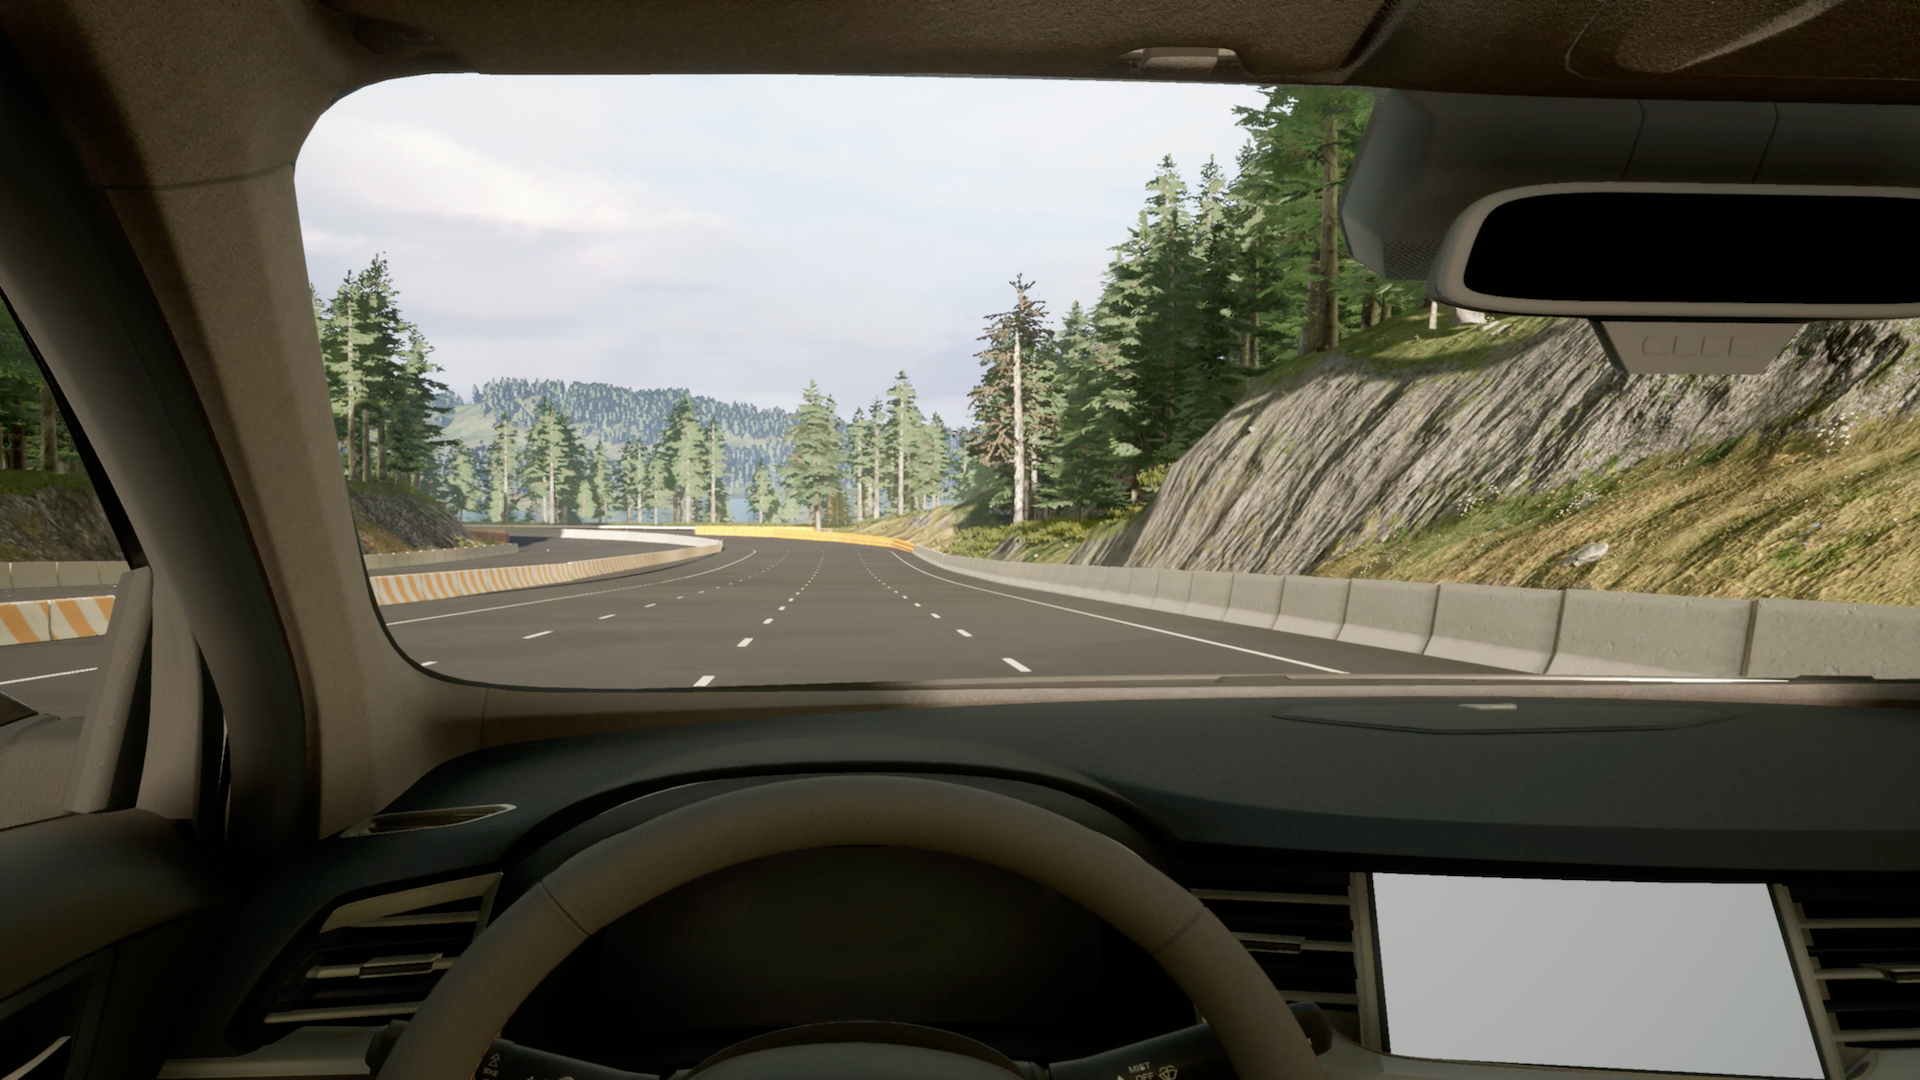
\includegraphics[width=1.0\columnwidth]{simulator}
  \caption{Cockpit view screenshot of the real-time driving simulator giving a glimpse on the graphical quality and realism.}
\end{figure}

% - - - - - - - - - - - - - - - - - - - - - - - - - - - - - - - - - - - - - - -

\section{Impact}

The free and open-source \Acme{} library provides users quick and easy access to the manipulation of geometric entities. It has been successfully used in the tire-road interaction computation. A first version of the library was developed in~\cite{stocco2019valutazione} and was planned to be used coupled with H. Pacejka \emph{Magic Formulae}~\cite{pacejka2012tire} tire model for online time-optimal motion planning and control of vehicle applications~\cite{piccinini2022predictive}.

The library has a \Matlab{} \Mex{} wrapper that allows less experienced developers to exploit the software core while maintaining low programming language complexity. In case it was decided on a \cpp{} interface, the library allows you to quickly develop efficient, memory safe and low verbose code. The usage of the \Collection{} object, combined with the \AabbTree{} and the heavy usage of smart pointers allows to perform fast collision detection, intersection and sorting on a large set of (potentially heterogeneous) objects of type \Entity{}. Above all, from what is known to the authors, \Acme{} is the only library that has the same polymorphic behaviour in both the \cpp{} interface and the \Matlab{} \Mex{} wrapper. Moreover, other state-of-the-art geometry libraries like those mentioned in Section \ref{sec:1} do not guarantee double compatibility between \cpp{} and \Matlab{} environments.

% - - - - - - - - - - - - - - - - - - - - - - - - - - - - - - - - - - - - - - -

\section{Conclusions}

The world of simulation is always in evolution. The ability to keep a minimum stable core is a key feature for a less concerned future developments. \Acme{} library is a very basic and easy-to-use \cpp{} geometry library that aims to be a minimal tool for real-time applications. The peculiarity that makes this library simple but at the same time effective is the presence of a minimum set of basic entities data types together with \AabbTree{} and \Collection{} objects. The user can work with a large number of object instances in an efficient way. The library allows to efficiently create, intersect, and destroy basic geometry entities. \Acme{} is thus convenient for both a simple collision detection work and a more time expensive intersection evaluation. The object-oriented design allows experienced programmers to extend the library if needed. Thorough documentation on both \cpp{} and \Matlab{} APIs, together with a set of step-by-step examples complete this tool. An example of library extension and practical usage has been shown in Section \ref{example}. In its current version, the library is in fact very keen on representing tires and road surfaces respectively modelled by a multitude of \Triangle{}\textsc{s} and a set of \Disk{} objects, and it has been tested on a real-time driving simulator. In order to guarantee performance and stability, the library has been accessed in high density mesh locations and extreme cases. Even if the natural habitat of \Acme{} is in driving simulation, we believe that it may serve also for generic third-party projects involving collision detection and intersection evaluation of large sets of basic or compositions of geometrical entities.


